\documentclass[12pt,a4paper]{article}
\usepackage[utf8]{inputenc}
\usepackage[T1]{fontenc}
\usepackage[english]{babel}
\usepackage[top=2cm, bottom=3cm, left=1.75cm, right=1.75cm]{geometry}
\usepackage{placeins}
\usepackage{graphicx}
\usepackage{subfig}
  \graphicspath{{./figures/}}
\usepackage[unicode=true, bookmarks=true, bookmarksnumbered=true, bookmarksopen=true, bookmarksopenlevel=1, breaklinks=false, pdfborder={0 0 0}, pdfborderstyle={}, backref=page, colorlinks=true, linkcolor=blue, urlcolor=blue]{hyperref}
  \hypersetup{
      pdftitle={Green Beard with a nasty gene},
      pdfauthor={Antonino Orofino, Mathieu Serandour},
      pdfsubject={Social Emergence in Complex System - Micro-Study},
      pdfkeywords={}
  }

\usepackage{array}
\newcolumntype{?}{!{\vrule width 2pt}}

\makeatletter
\def\hlinewd#1{%
\noalign{\ifnum0=`}\fi\hrule \@height #1 \futurelet
\reserved@a\@xhline}
\makeatother

\usepackage{listings}
\usepackage{xcolor}
\definecolor{darkred}{rgb}{0.6,0.0,0.0}
\definecolor{darkgreen}{rgb}{0,0.50,0}
\definecolor{lightblue}{rgb}{0.0,0.42,0.91}
\definecolor{orange}{rgb}{0.99,0.48,0.13}
\definecolor{grass}{rgb}{0.18,0.80,0.18}
\definecolor{pink}{rgb}{0.97,0.15,0.45}
% General Setting of listings
\lstset{
  aboveskip=1em,
  breaklines=true,
  abovecaptionskip=6pt,
  captionpos=b,
  escapeinside={\%*}{*)},
  frame=single,
  numbers=left,
  numbersep=15pt,
  numberstyle=\tiny,
}
% 0. Basic Color Theme
\lstdefinestyle{colored}{ %
  basicstyle=\ttfamily,
  backgroundcolor=\color{white},
  commentstyle=\color{green}\itshape,
  keywordstyle=\color{blue}\bfseries\itshape,
  stringstyle=\color{red},
}
% 1. General Python Keywords List
\lstdefinelanguage{PythonPlus}[]{Python}{
  morekeywords=[1]{,as,assert,nonlocal,with,yield,self,True,False,None,} % Python builtin
  morekeywords=[2]{,__init__,__add__,__mul__,__div__,__sub__,__call__,__getitem__,__setitem__,__eq__,__ne__,__nonzero__,__rmul__,__radd__,__repr__,__str__,__get__,__truediv__,__pow__,__name__,__future__,__all__,}, % magic methods
  morekeywords=[3]{,object,type,isinstance,copy,deepcopy,zip,enumerate,reversed,list,set,len,dict,tuple,range,xrange,append,execfile,real,imag,reduce,str,repr,}, % common functions
  morekeywords=[4]{,Exception,NameError,IndexError,SyntaxError,TypeError,ValueError,OverflowError,ZeroDivisionError,}, % errors
  morekeywords=[5]{,ode,fsolve,sqrt,exp,sin,cos,arctan,arctan2,arccos,pi, array,norm,solve,dot,arange,isscalar,max,sum,flatten,shape,reshape,find,any,all,abs,plot,linspace,legend,quad,polyval,polyfit,hstack,concatenate,vstack,column_stack,empty,zeros,ones,rand,vander,grid,pcolor,eig,eigs,eigvals,svd,qr,tan,det,logspace,roll,min,mean,cumsum,cumprod,diff,vectorize,lstsq,cla,eye,xlabel,ylabel,squeeze,}, % numpy / math
}
% 2. New Language based on Python
\lstdefinelanguage{PyBrIM}[]{PythonPlus}{
  emph={d,E,a,Fc28,Fy,Fu,D,des,supplier,Material,Rectangle,PyElmt},
}
% 3. Extended theme
\lstdefinestyle{colorEX}{
  basicstyle=\ttfamily,
  backgroundcolor=\color{white},
  commentstyle=\color{darkgreen}\slshape,
  keywordstyle=\color{blue}\bfseries\itshape,
  keywordstyle=[2]\color{blue}\bfseries,
  keywordstyle=[3]\color{grass},
  keywordstyle=[4]\color{red},
  keywordstyle=[5]\color{orange},
  stringstyle=\color{darkred},
  emphstyle=\color{pink}\underbar,
}
\lstset{style=colorEX}

\newcommand{\parag}[1]{
  \vspace{8mm}
  \noindent
  {\LARGE\textbf{#1}}
  \vspace{3mm}
}
\newcommand{\A}{\textbf{ANTONINO}\\}
\newcommand{\M}{\textbf{MATHIEU}\\}

\begin{document}

\begin{center}
  \begin{tabular}{|p{0.2\textwidth}|p{0.75\textwidth}|}
    \hline
    {
    \vspace{0cm} % without it, bugs, don't know why?
    \centerline{
\includegraphics[width=\linewidth]{tp-ipp}}
    }
    & {
      \vspace{0cm} % same here
      \centering
      \large
      {\hfill November, 2021}
      
      \vspace*{.5cm}
      ATHENS course : \textbf{TP-09}
      
      \vspace*{.5cm}
      {\LARGE\textbf{Social Emergence in Complex System}}
      
      \vspace*{.5cm}
      Micro-study

      \vspace*{1.5cm}
      \hfill\href{http://teaching.dessalles.fr/SECS}{\ttfamily teaching.dessalles.fr/SECS}
      }\\
    \hline
  \end{tabular}
\end{center}

Names:	\textbf{Antonino Orofino} and \textbf{Mathieu Serandour}

\vspace{5mm}
\hrule width \hsize \kern .5mm \hrule width \hsize height .5pt
\vspace{4mm}

\begin{center}
{\LARGE\textbf{Green Beard with a nasty gene}}
\end{center}

\vspace{-4mm}
\parag{Abstract}

Having a certain characteristic is usually either good or bad for an individual, however, this isn't always true. Indeed, there can be features for which the dividing line between benefits and obstacles is not so defined.
We focused our study in analysing this scenario. In particular, we studied the conditions that led to the spread or disappearance of these kind of features.

\parag{Problem}

We thought that a feature can be profitable, but still not accepted by peers. For example, having a green beard and being altruistic with other green beard carriers is profitable as we saw in the lab, though it can lead to secondary effects: people might find you less attractive or mock your beard. We wanted to study if the gene that carries a feature like this one could prevail even though it leads to push back from another part of the population, and what conditions rule.

\parag{Method}

\A
We chose to begin with the scenario "GreenBeard". First of all, we added a new gene called 'Nasty'. Both the GreenBeard gene and the Nasty one are represented by a single bit. According to the genes' values there can be 3 kinds of agents:
\begin{itemize}
  \setlength\itemsep{0.5mm}
  \item \textbf{Green Beard carriers}: an agent with only the GreenBeard gene;
  \item \textbf{Nasty carriers}: an agent with only the Nasty gene;
  \item \textbf{GreenBeard-Nasty carriers}: an agent who has both genes.
\end{itemize}
Actually there is also a fourth kind of individual: the one with neither one of two genes.

In order to understand the model we should analyse what happen to an individual when he meet another agent. Each behaviour is related to the genes.
\begin{itemize}
  \item \textbf{Green Beard carriers}\\
    - altruist among other green beard carriers.
  \item \textbf{Nasty individuals}\\
    - hate the Green Beard carriers, so steal scores from them by attacking them;\\
    - they receive a penalty for being nasty.
  \item \textbf{GreenBeard-Nasty carriers}\\
    - receive a penalty for have betrayed another agent of the same group.
\end{itemize}

\M
The original scenario only had two parameters: \texttt{GB\_cost} and \texttt{GB\_gift}. These parameters are used to control the value/cost of being altruist among GreenBeard carriers.
Then we added other 4 parameters:
\begin{itemize}
  \setlength\itemsep{0.5mm}
  \item \texttt{N\_Payback} defines the payback for a nasty after attacking a GreenBeard carrier;
  \item \texttt{N\_Attack} defines the cost for a GreenBeard carrier for being attacked;
  \item \texttt{N\_Penalty} is used to specify the penalty given to a Nasty individual for behaving in a bad way;
  \item \texttt{GB\_N\_Penalty} defines the penalty given to a GreenBeard carrier for behaving nastily to anther individual of the same group.
\end{itemize}
These parameters were added both in \texttt{EvolifeConfigTree.xml} and \texttt{Expe/GreenBeard.evo} file.\\

\A
We can summarize all interactions behaviours in table \ref{table:payoff}. Let's consider an interaction between an individual and a partner. We represent the individual using columns while the rows for the partner. The cell identified by the individuals couple give us the payoff (or cost if negative) for both the agents that meet each other. 

\bgroup
\def\arraystretch{1.5}
\begin{table}[h!]
\centering
\begin{tabular}{  c ? c | c }
 & \textbf{GreenBeard} & \textbf{Non-GreenBeard} \\ 
 \hlinewd{2pt}
 \textbf{GreenBeard} & \footnotesize{(-GB\_Cost,GB\_Gift)} & \footnotesize{(0,0)} \\  
 \hline
 \textbf{Nasty} & \footnotesize{(N\_Payback - N\_Penalty, - N\_Attack)} & \footnotesize{(-N\_Penalty,0)} \\
 \hline 
 \textbf{Nasty-GreenBeard}& \footnotesize{(N\_payback - N\_Penalty -GB\_N\_Penalty, - N\_Attack)} & \footnotesize{(-N\_Penalty,0)}
\end{tabular}
\caption{\label{table:payoff}Payoff table}
\end{table}
\egroup

\noindent To implement this logic, we chose to overload the \texttt{interaction} function in \texttt{S\_GreenBeard.py}.
\begin{lstlisting}[language=Python, caption=Overloading of \texttt{interaction} function]
  def interaction(self, indiv, partner):
    """ Genes control the behaviour of 'indiv' toward 'partner'
    """
    if (not indiv.gene_value('GreenBeard')) and indiv.gene_value('Nasty') and partner.gene_value('GreenBeard'):
      indiv.score(self.Parameter('N_Payback'))
      partner.score(-self.Parameter('N_Attack'))
    elif indiv.gene_value('GreenBeard') and (not indiv.gene_value('Nasty')) and partner.gene_value('GreenBeard'):
      indiv.score(-self.Parameter('GB_Cost'))
      partner.score(self.Parameter('GB_Gift'))
    elif indiv.gene_value('GreenBeard') and indiv.gene_value('Nasty') and partner.gene_value('GreenBeard'):
      indiv.score(self.Parameter('N_Payback'))
      indiv.score(-self.Parameter('GB_N_Penalty'))
      partner.score(-self.Parameter('N_Attack'))
    if indiv.gene_value('Nasty'):
      indiv.score(-self.Parameter('N_Penalty'))
\end{lstlisting}

\M
Finally, we thought of adding a new feature that would make our model closer to reality. In real life, in fact, a GreenBeard carrier would not choose a Nasty individual as a partner for reproduction.
In order to reach this goal we added another parameter, called \texttt{N\_Segregation}, and overload the method \texttt{parents} only if this parameter is \texttt{True}.

\begin{figure}[h]
    \centering
    \frame{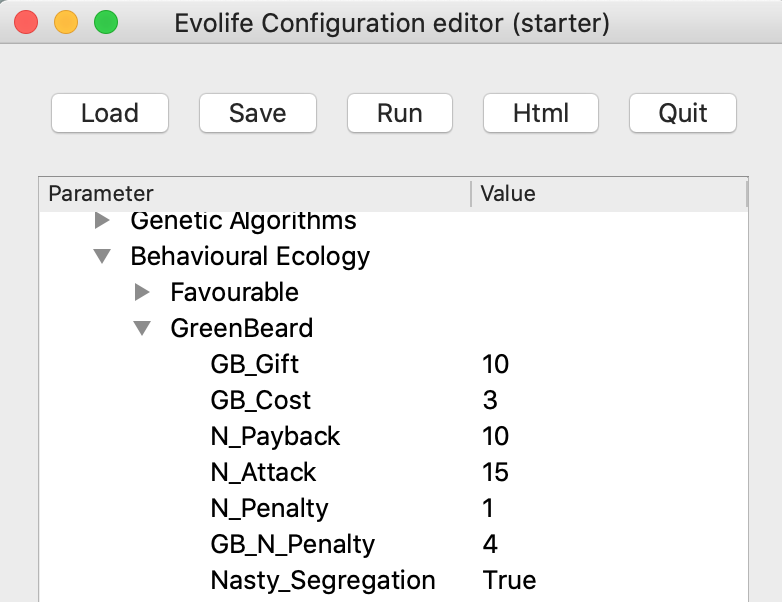
\includegraphics[width=8cm]{param}}
    \caption{\label{fig:4} List of the parameters in Evolife}
\end{figure}

\begin{lstlisting}[language=Python, caption=Overloading of \texttt{parents} function]
  def parents(self, candidates):
    """
    If it is set to True, then GreenBeard carriers will not reproduce with nasty carriers.
    """
    if not self.Parameter('Nasty_Segregation'):
      return super().parents(candidates)
    try:  
      for i in range(10):
        m = random.choice(candidates)
        f = random.choice(candidates)
        if m[0].gene_value('Nasty') and f[0].gene_value('GreenBeard'):
          continue
        if f[0].gene_value('Nasty') and m[0].gene_value('GreenBeard'):
          continue
        return (m,f)
      return None
    except  IndexError: return None
\end{lstlisting}

\vspace{-1cm}
\parag{Results}

In all the results, the red curve represents the rate of nasty gene in the population while the red one represents the rate of green beard carriers. We chose to make all the tests with a \texttt{Selectivity} value of 10 and no \texttt{SelectionPressure}, as we saw in the lab that it promotes altruism.

\begin{figure}[htp] 
    \centering
    \subfloat[Graph]{%
        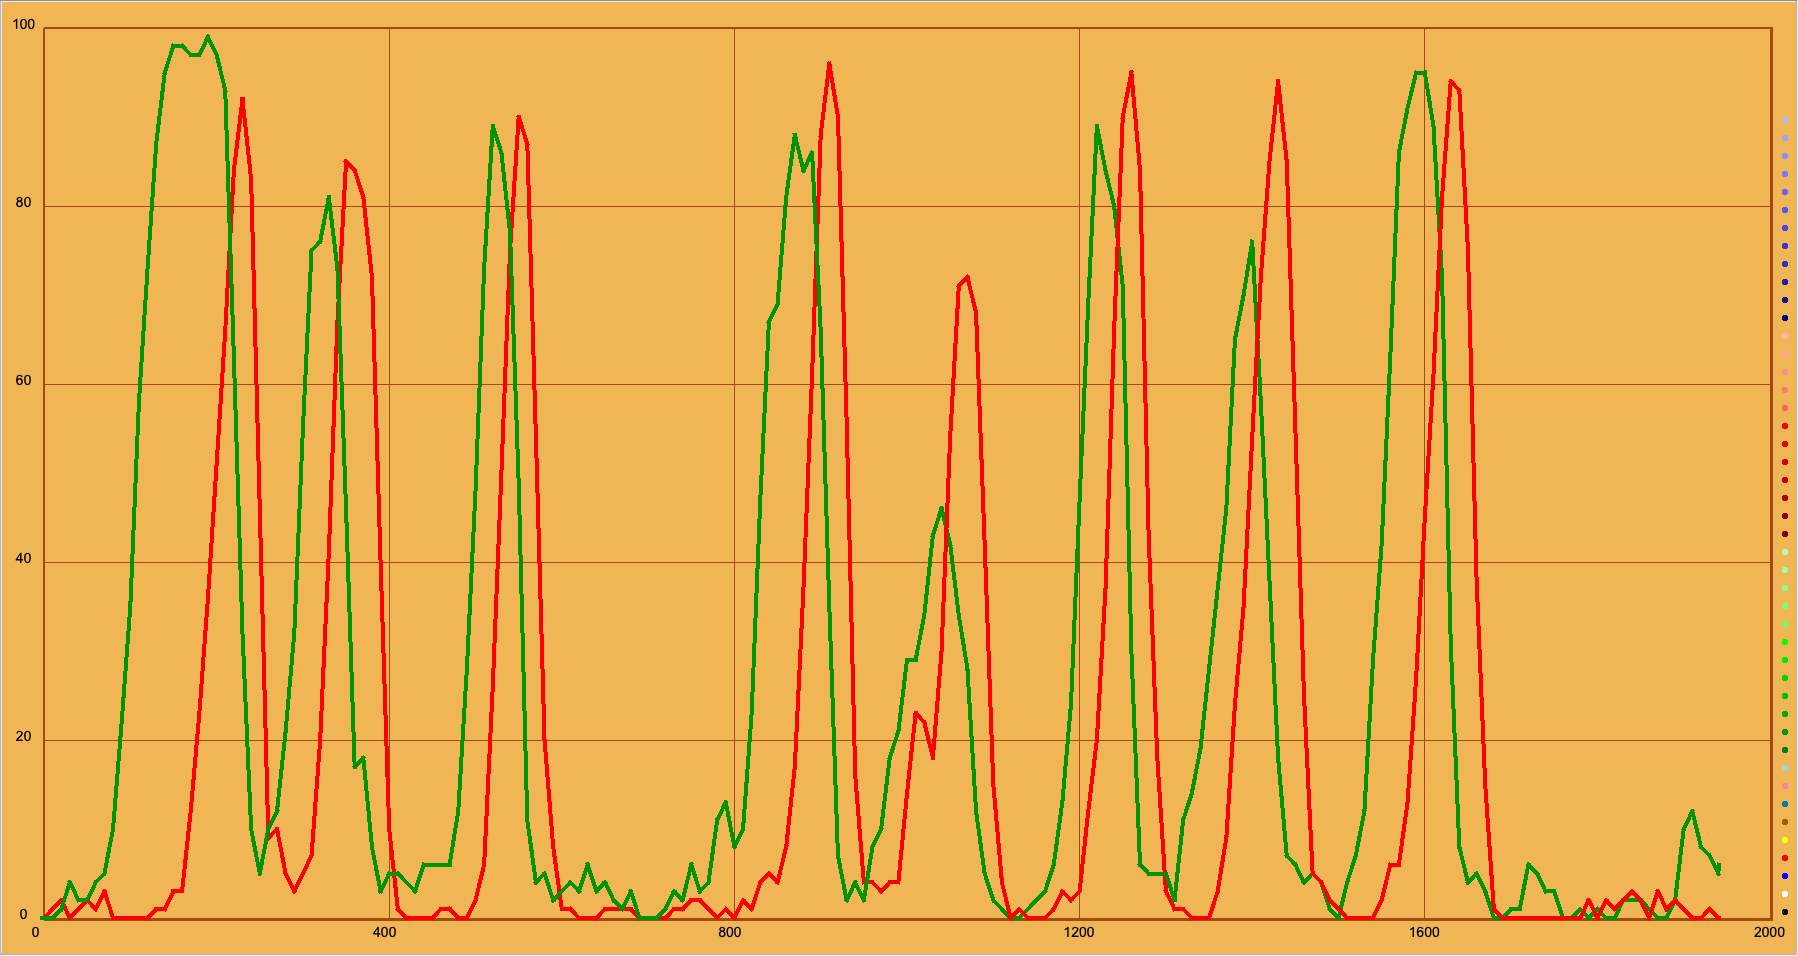
\includegraphics[width=0.65\textwidth]{1}%
        \label{fig:1}%
        }%
    \hfill%
    \subfloat[Parameters]{%
        \frame{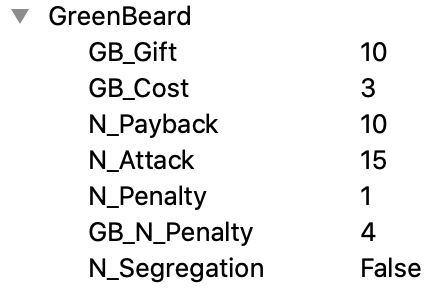
\includegraphics[width=0.3\textwidth]{1_param}}%
        \label{fig:1_param}%
        }%
    \caption{Spread of the genes with \texttt{N\_Segregation} effect}
\end{figure}

\begin{figure}[htp] 
    \centering
    \subfloat[Graph]{%
        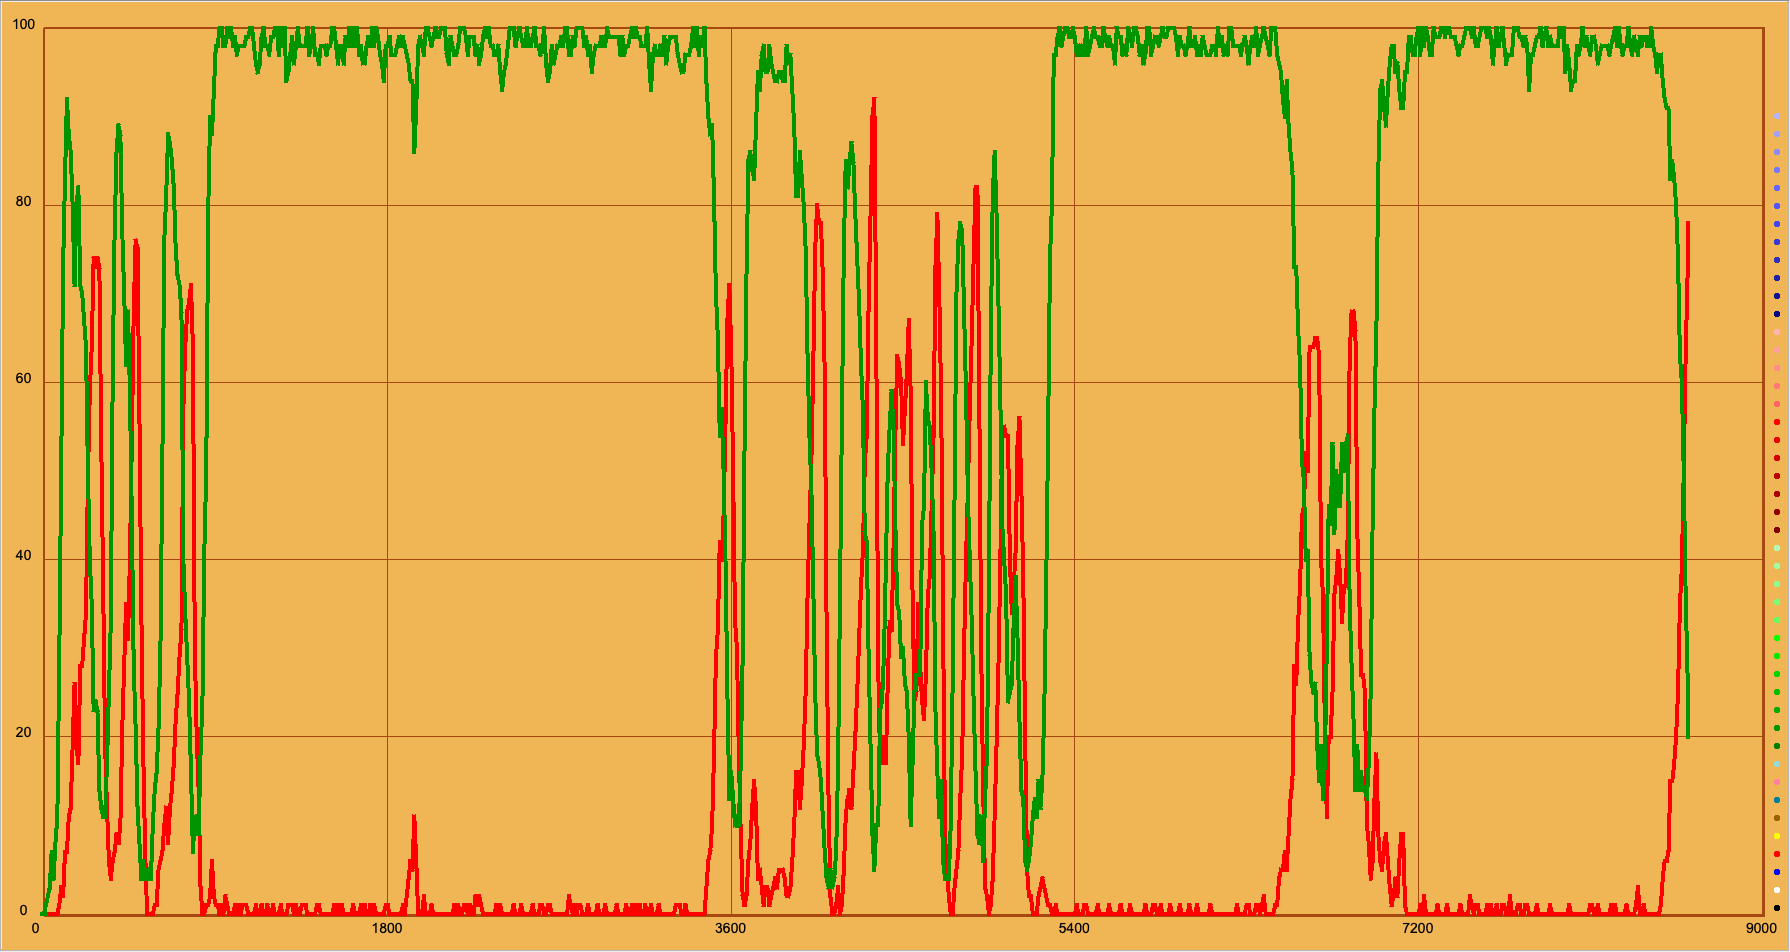
\includegraphics[width=0.65\textwidth]{2}%
        \label{fig:2}%
        }%
    \hfill%
    \subfloat[Parameters]{%
        \frame{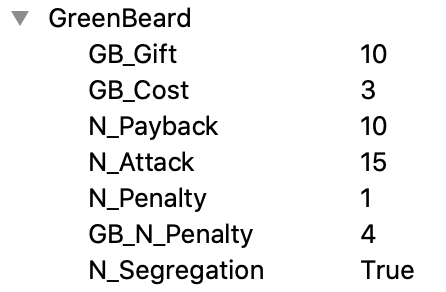
\includegraphics[width=0.3\textwidth]{2_param}}%
        \label{fig:2_param}%
        }%
    \caption{Spread of the genes without \texttt{N\_Segregation} effect}
\end{figure}

\begin{figure}[htp] 
    \centering
    \subfloat[Graph]{%
        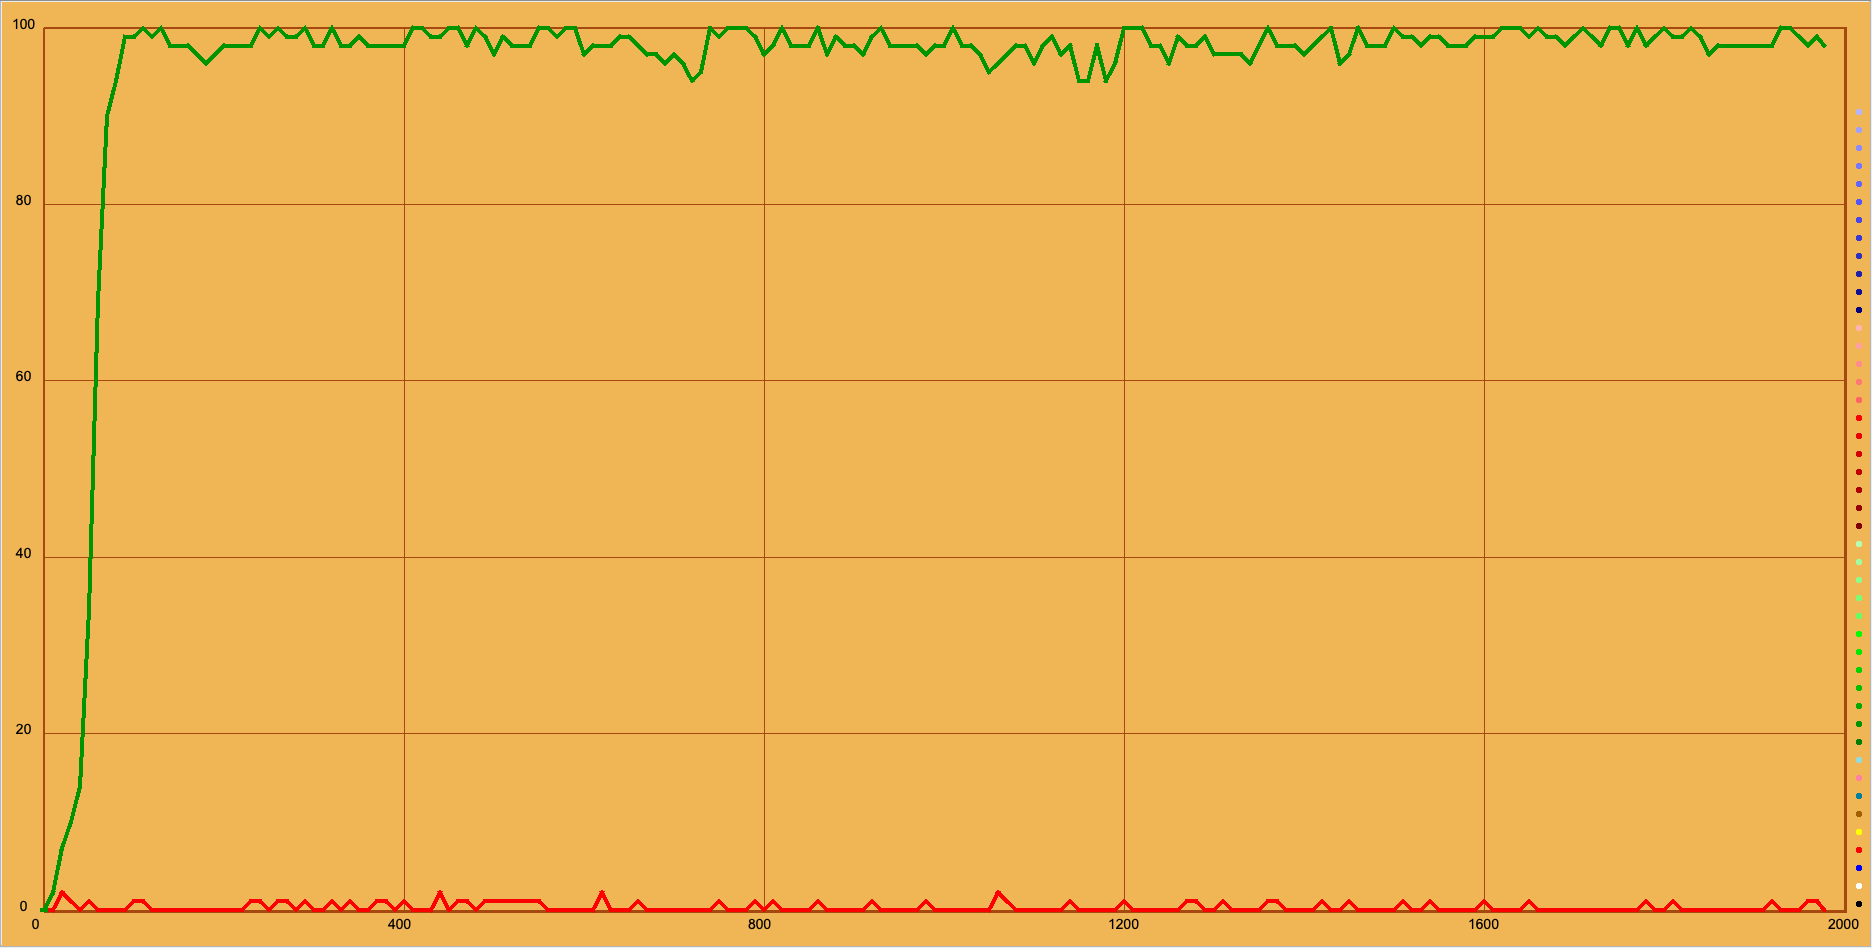
\includegraphics[width=0.65\textwidth]{3}%
        \label{fig:3}%
        }%
    \hfill%
    \subfloat[Parameters]{%
        \frame{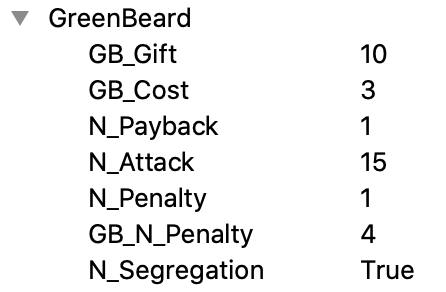
\includegraphics[width=0.3\textwidth]{3_param}}%
        \label{fig:3_param}%
        }%
    \caption{Spread of the genes with a low \texttt{N\_Payback}}
\end{figure}

\begin{figure}[htp] 
    \centering
    \subfloat[Graph]{%
        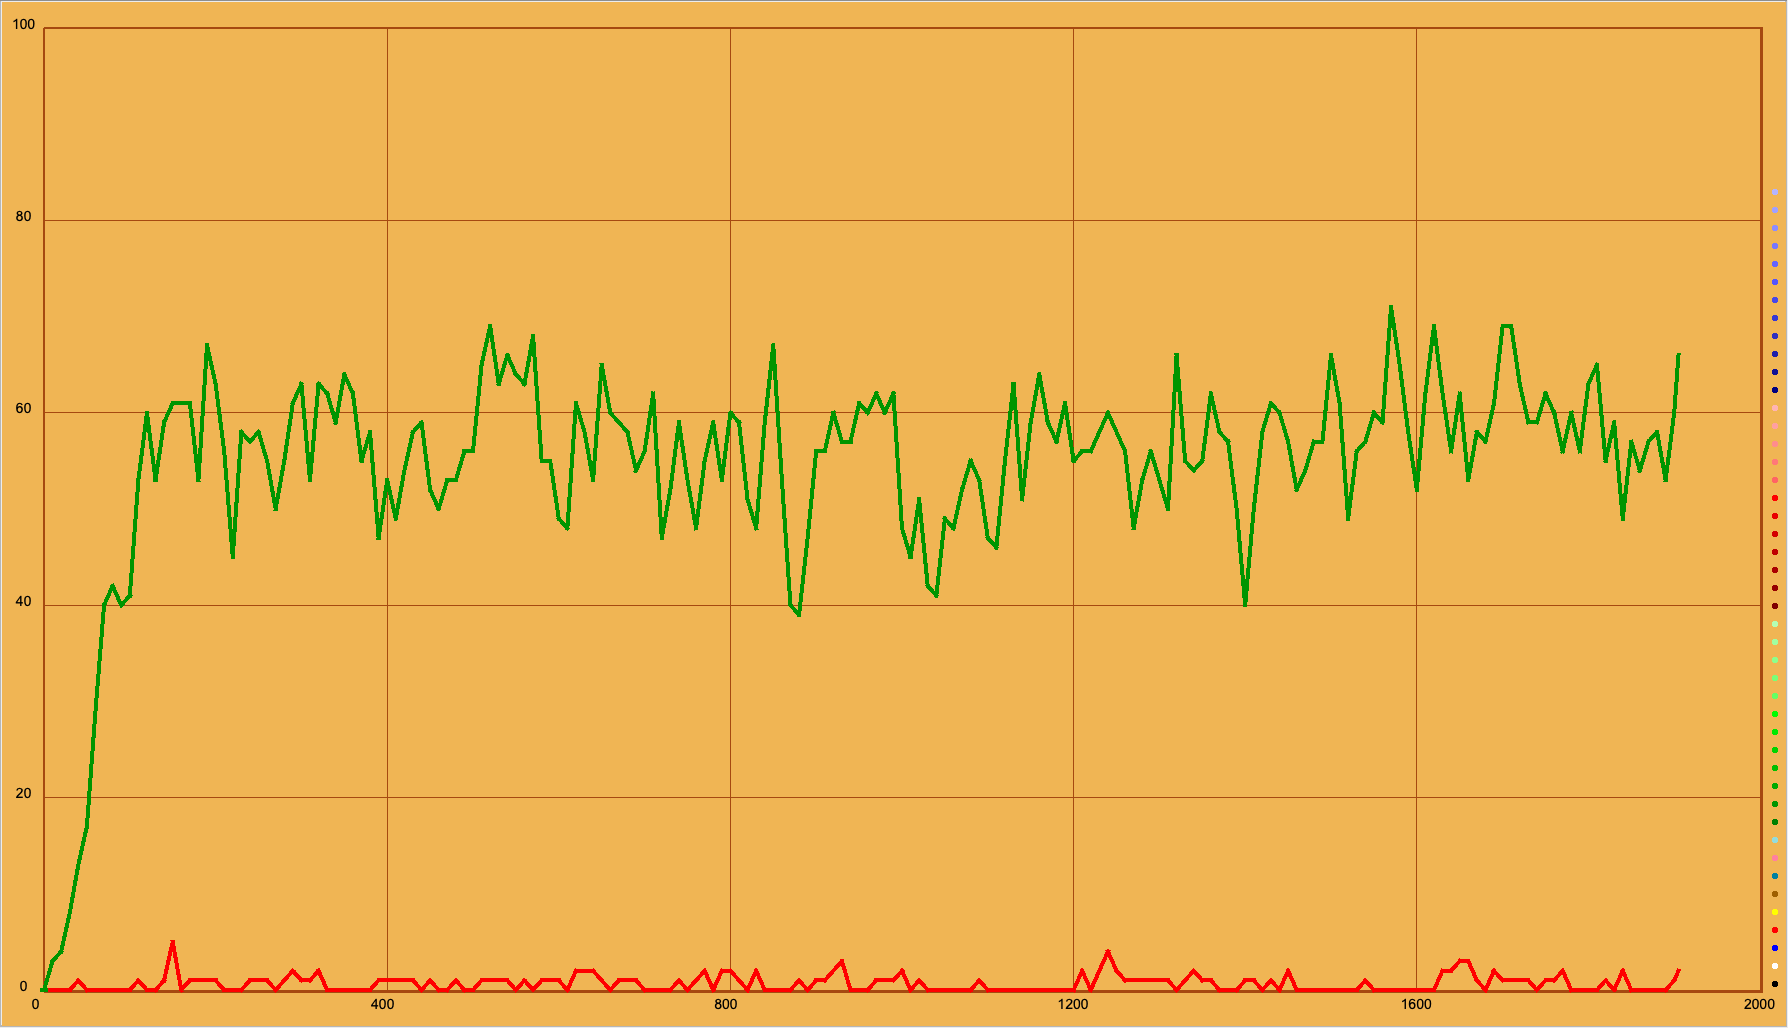
\includegraphics[width=0.65\textwidth]{4}%
        \label{fig:4}%
        }%
    \hfill%
    \subfloat[Parameters]{%
        \frame{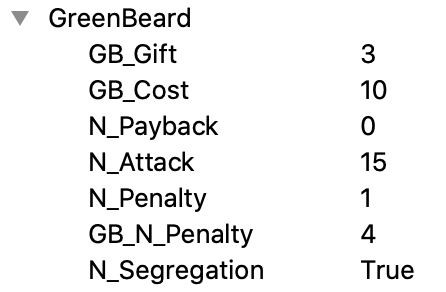
\includegraphics[width=0.3\textwidth]{4_param}}%
        \label{fig:4_param}%
        }%
    \caption{Spread of the genes with \texttt{N\_Payback} equals to zero and \texttt{GB\_Cost} > \texttt{GB\_Gift}}
\end{figure}

\begin{figure}[htp] 
    \centering
    \subfloat[Graph]{%
        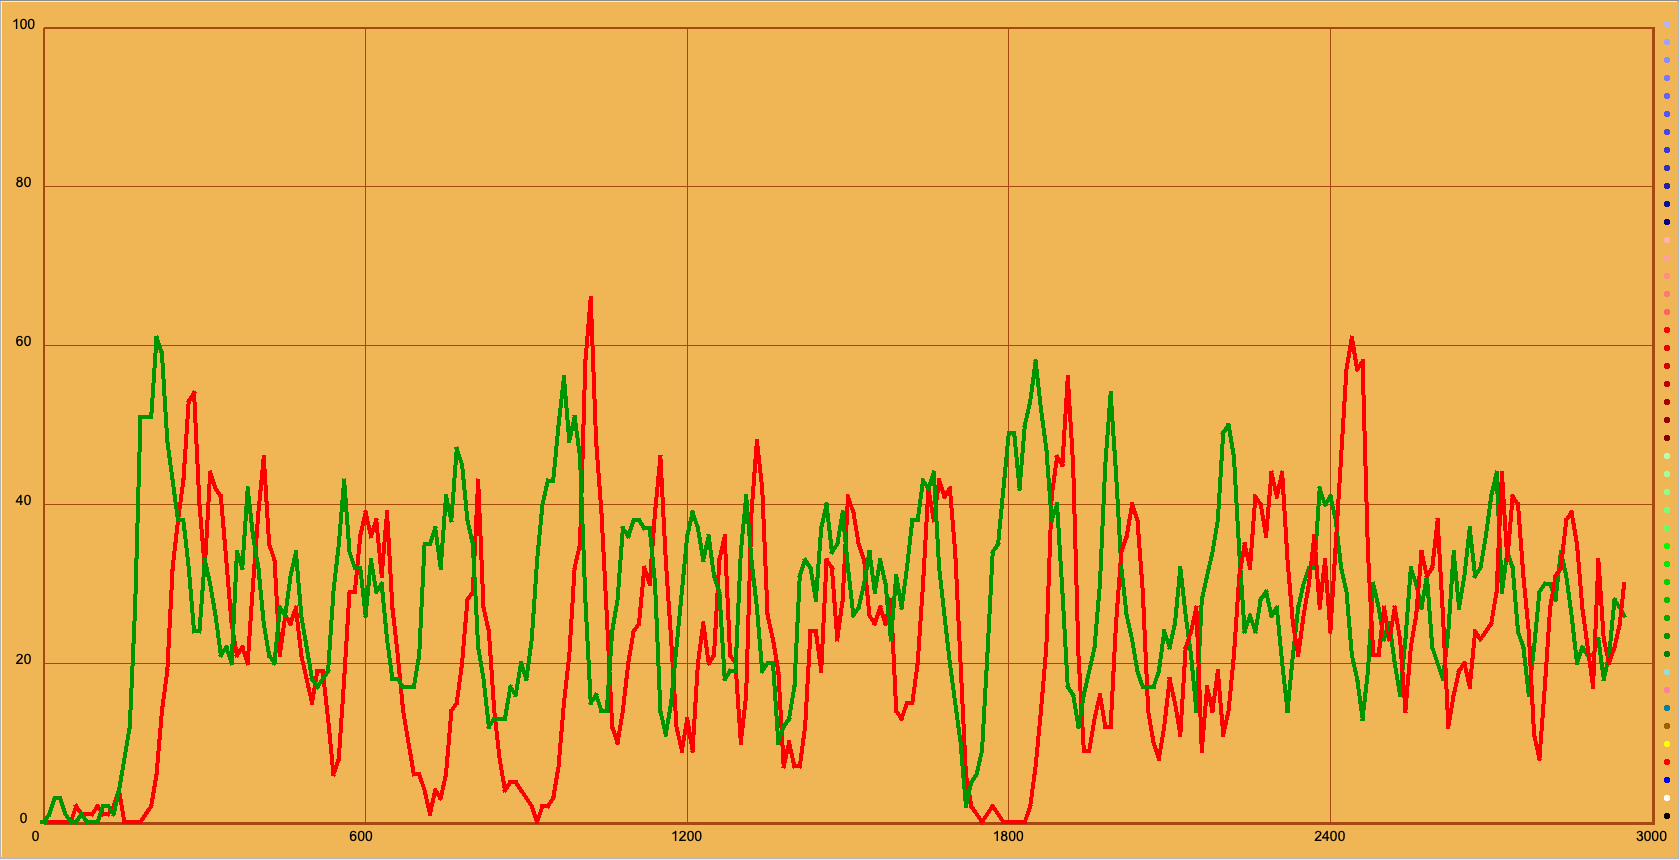
\includegraphics[width=0.65\textwidth]{5}%
        \label{fig:5}%
        }%
    \hfill%
    \subfloat[Parameters]{%
        \frame{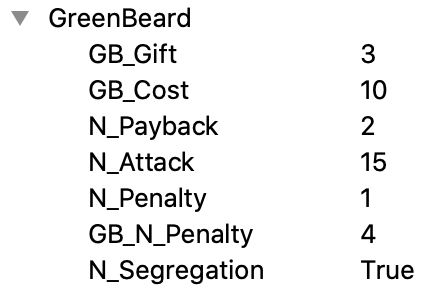
\includegraphics[width=0.3\textwidth]{5_param}}%
        \label{fig:5_param}%
        }%
    \caption{Spread of the genes with a bit of \texttt{N\_Payback} ( > \texttt{N\_Penalty}) and \texttt{GB\_Cost} > \texttt{GB\_Gift}}
\end{figure}

\FloatBarrier
\parag{Discussion}

\A

\noindent\textbf{Figure \ref{fig:1}}
\vspace{1.5mm}

If there is too few green beard carrier in the population, we expect the red curve to fall as there is no one to be nasty against, and being nasty has a cost. We also expect the red curve to rise if there is enough green beard carriers, as it is profitable to be nasty if there is a lot of individuals to be nasty against.

As the put a gift way bigger than the cost for the green beard carriers, we also expect that the green curve rises up as long as the red one is not too high. Thus, we expected an oscillating behaviour.

The results are quite similar to our expectations. However, We were surprised to observe that the sum of the two curves was higher than 100: it means that a non negligible proportion of the population presents both genes. It is surprising because the penalty for being both nasty and green beard carrier was quite high: \texttt{GB\_N\_Penalty=4} and \texttt{N\_Penalty=1}.

\vspace{5mm}
\noindent\textbf{Figure \ref{fig:2}}
\vspace{1.5mm}

It seems more intuitive to us that the nasty individuals don’t want to reproduce with the green beard carriers, that is why we added the \texttt{N\_Segregation} parameter. When setting it to True, we could expect that if the green beard carriers dominates the population, it would be hard for nasty individuals to appear as they don’t reproduce with green beard carrier.

The results are quite similar to the the last during some intervals: the two genes struggle to dominate the other, but eventually the green beard gene becomes dominant and prevails for a pretty long time. When it eventually decays due to random mutations, the struggling comes back.

We were surprised to see that the sum of the two curves always is 100: this time, no one have both genes, which is explainable because no nasty individual reproduces with a green beard carrier and the penalty for being both nasty and green beard carrier is still high. The surprising fact is that no one don’t present any of the two genes. It is always better to be either nasty or green beard carrier than to be neutral.

\vspace{1cm}
\M

\noindent\textbf{Figure \ref{fig:3}}
\vspace{1.5mm}


We tried to put a high value of the nasty stealing for the green beard carriers along with a small value for the their payoff. At first sight, we expected some struggling between the two genes still as the payback was equal to the penalty for being nasty, so being nasty should be neutral when the green beard rate is very high. Besides, the presence of nasty individuals should still diminish the number of green beard carriers. Though we observe that the red curve never goes above zero. This is because the altruism of the green beard gene is more beneficial than being neutral.

We obtained the exact same curves when putting different values to \texttt{N\_Payback}, up to 9. Though we expected that some nasty individuals would remain as their payback is superior to the penalty. This is because we put \texttt{Selectivity} to 10 and \texttt{SelectionPressure} to 0: this configuration promotes elitism and therefore the green beard carriers that did not cross any nasty individual but got gifts from other green beard carriers would gain more than the nasty individuals would get from steeling.

\vspace{5mm}
\noindent\textbf{Figure \ref{fig:4}}
\vspace{1.5mm}

This curve is a reminder of what we observed in the corresponding lab. When \texttt{GB\_Cost} < \texttt{GB\_Gift} for the green beard carriers, we would expect the green curve to stay to 0, but we observe that around 60\% of the population presents the green beard gene. We get the same curves if the the gift is very low. This is for the same reason as the preceding discussion: the \texttt{Selectivity} parameter promotes elitism. A few green beard carriers get gifts and never give some. They still get points so they get sectioned.

\vspace{5mm}
\noindent\textbf{Figure \ref{fig:5}}
\vspace{1.5mm}

Figure 5 shows that when the natural selection promotes elitism, an altruism gene can prevail even when the Cost is superior the the Gift. Figure 2 also shoes that the altruism gene can prevail even when the altruist individuals are targets to nasty behaviour.

Figure 6 is an interesting curve: it shoes that when we sum these two factors: a cost superior to the gift and nasty behaviours against green beard carriers, altruism is impacted. We put a small payback, and observe that the green curve is much lowered in comparison to Figure 5. This is because even though selection is done in an elitism manner, fewer individuals both get gifts and never cross any nasty individual.

To conclude, in the case we focused on: nasty individuals don’t reproduce with altruist green beard carriers, we can say that the condition that assures that altruism prevails is that the gift is higher to the cost. When it is not the case, as long as nasty individuals get satisfaction from bullying the altruists, altruism is to diminish.

% \parag{Bibliography}

% All useful references with links.


\end{document}
